\documentclass{article}
\usepackage{amsfonts}
\usepackage{amsthm}
\usepackage{amssymb}
\usepackage{amsmath}
\usepackage{graphicx}
\usepackage{subcaption}
\usepackage[shortlabels]{enumitem}
\usepackage{xcolor}
\usepackage{tikz}

\newcommand{\new}[1]{
    \vspace{2mm}
    \noindent
    \textbf{
    \underline{#1}}
}

\def\calO{{\mathcal{O}}}
\def\th{{\theta}}
\def\_{{\hspace{1mm}}}
\def\<{{\langle}}
\def\>{{\rangle}}


\newcounter{problemcnt}
\setcounter{problemcnt}{0}

\newcommand{\Problem}{{
    \vspace{5mm}
    \stepcounter{problemcnt}
    \noindent
    \arabic{problemcnt}. 
}
}

\newcommand{\nProblem}[1]{
    \vspace{5mm}
    \noindent
    \setcounter{problemcnt}{#1}
    \arabic{problemcnt}. 
}


\newcommand{\Proof}{{
    \vspace{2mm}
    \noindent
    \textbf{
    \underline{Proof}}
}
}

\newcommand{\textOr}{
    {
        \hspace{5mm}
        \textrm{or}
        \hspace{5mm}
    }
}

\newcommand{\textAnd}{
    {
        \hspace{5mm}
        \textrm{and}
        \hspace{5mm}
    }
}

\newcommand{\m}{
    \cdot
}

\newcommand{\Pt}[1]{
    $P_{#1}$
}

\newcommand{\Szpt}[1]{
    $|P_{#1}|$
}

\newcommand{\bbinom}[2]{
    \bigg(\binom{#1}{#2}\bigg)
}



\begin{document}
\begin{center}
\LARGE
Combinatorics HW4

\Large
Daniel Son
\end{center}


Section 4.6: 36, 37, 43, 50

Section 5.7: 3, 4, 7, 9, 15, 23, 24


\new{Additional Problem 1.}
 Draw the Hasse diagram for the divides rela-
tion on the positive divisors of 30. Then explain in your own words the
relationship between that diagram, and the diagram in Figure 4.7 from
the textbook.

\new{Solution}

\begin{center}
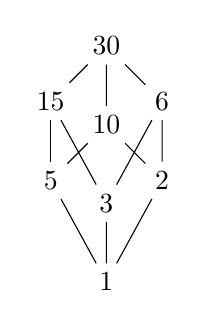
\begin{tikzpicture}
    \node(top) {$30$};
    \node(15)[below left of=top] {$15$};
    \node(10)[below of=top]{$10$};
    \node(6)[below right of=top]{$6$};
    \node(2)[below of=6] {$2$};
    \node(3)[below of=10] {$3$};
    \node(5)[below of=15]{$5$};
    \node(1)[below of=3]{$1$};
    \draw (top) -- (15) -- (3) -- (1) -- (2) -- (6) -- (top);
    \draw (15) -- (5);
    \draw (top) -- (10) -- (5) -- (1);
    \draw (3) -- (6);
    \draw (2) -- (10);
\end{tikzpicture}
\end{center}

The Hasse diagram of the divisors of 30 are isomorphic to the 
Hasse diagram of the subsets of $\{1, 2, 3\}$. We can describe the 
isomorphism as follows. Let define function $f$ to as $f(1) = 2, 
f(2) = 3, f(3) = 5$. The isomorphism $\phi$ that maps subsets 
to numbers is
\[
    \phi(S) = \prod_{k \in S} f(k) 
\]
where $S \subseteq \{1,2, 3\}$. For example, 
$\phi(\{1, 3\}) = f(1)\m f(3) = 2\times 5 = 10$. By the 
fundamental theorem of arithmetic, it is easy to see that 
each divisor correspond to a unique subset via the inverse of 
$\phi$. \hfill \qed

\new{Sec4.6Q36} 
Let X be a set of n elements. How many different relations on X are there? How 
many of these relations are reflexive? Symmetric? Antisymmetric? Reflexive 
and symmetric? Reflexive and anti-symmetric?

\new{Solution}
We distinguish any ordered pairs of two integers into distinct 
and nondistinct pairs. The former refers to the pairs 
which have distinct entries. That is $(a, b)$ where $a \neq b$. 
The latter refers to $(a, a)$. 

Relations can be considered as a set of ordered pairs. If the 
relation is symmetric, the choice of a nondistinct pair of the 
relation forces the relation to include the corresponding pair. 
That is, if $(a, b) \in R$ for where $a \neq b$, then $(b, a) \in R$. 
The choice of nondistinct pairs does not affect the symmetry of 
the relation. For a relation to be reflexive, it must include 
all the nondistinct pairs. For a relation to be antisymmetric 
it must not include any of the nondistinct pairs. 

From the observations made above, we construct relations that satisfy 
the given conditions. If the relation is defined from the cannonical 
set $[n]$ to $[n]$, there exists n nondistinct pairs and $\binom{n}{2}$
couples of distinct pairs. 

To construct all the symmetric relations, we either choose or leave 
each nondistinct pair or a distinct couple of pairs. There 
are a total of $n + \binom{n}{2}$ such objects. Thus, the 
number of symmetric relations are $\boxed{2^{n(n+1)/2}}$. 

As for the reflexive relations, we choose all the nondistinct 
pairs and choose or leave the distinct pairs. There are $n(n+1)$ 
distinct pairs so we conclude that there are $\boxed{2^{n(n-1)}}$ 
reflexive relations. 

For antisymmetric relations, we can either choose or leave 
all the nondistinct pairs. For the distinct pair couples, we 
are allowed to choose one of the two pairs, or include both of 
them from the relation. Thus, there are three possible choices 
for each distinct couple. We count $\boxed{3^{\binom{n}{2}}2^n}$. 

For reflexive and symmetric relations, we choose or 
leave the distinct couples and choose all the nondistinct pairs. There 
are $\boxed{2^{n(n-1)/2}}$ such relations. 

For reflexive and antisymmetric relations, we choose all 
the nondistinct pairs and choose between the three options 
for each distinct couple. We count $\boxed{3^{\binom{n}{2}}}$.




\new{Sec4.6Q37} Let $R', R''$ be partial orders on a set $X$. 
Define the intersection $R$ such that $xRy \leftrightarrow (xR'y) \wedge 
(xR''y)$. Prove that $R$ is a partial order. 

\proof
We demonstrate symmetry, reflexivity, and transitivity of the relation 
$R$. For $R', R''$ are both partial orders, they must be reflexive. 
Hence, $xR'x$ and $xR''x$ for any $x \in X$. By the definition of 
the intersect $R$, $xRx$. $R$ is reflexive.

To demonstrate symmetry, assume $xRy$. We deduce $xR'y$ and $xR''y$ 
from definition. $R'$ and $R''$ are symmetric, so $yR'x$ and $yR''x$. 
Thus, $yRx$ and $R$ is symmetric. 

By the same logic, we demonstrate transitivity. Assume $xRy$ and $yRz$. 
$xR'y$ and $yR'z$ from the definition of $R$ and we infer $xR'z$ from 
the transitivity of $R'$. Likewise, $xR''z$. Thus, $xRz$ which concludes 
the proof. \hfill \qed


\new{Sec4.6Q43} Let $X = {a, b, c, d, e, f}$ and let the relation $R$ on X be defined by $aRb, b R c, 
c R d, aRe, e R f, f R d$. Verify that R is the cover relation of a partially ordered 
set, and determine all the linear extensions of this partial order. 

\end{document}